%%%%%%%%%%%%%%%%%%%%%%%%%%%%%%%%%%%%%%%%%%%%%%%%%%%%%%%%%%%%%%%%%%%%%%%%%%%%%%%%%%%%%%%
%%%%%%%%%%%%%%%%%%%%%%%%%%%%%%%%%%%%%%%%%%%%%%%%%%%%%%%%%%%%%%%%%%%%%%%%%%%%%%%%%%%%%%%
% 
% This top part of the document is called the 'preamble'.  Modify it with caution!
%
% The real document starts below where it says 'The main document starts here'.


\documentclass[12pt]{article}

\usepackage{amssymb,amsmath,amsthm}
\usepackage[top=1in, bottom=1in, left=1.25in, right=1.25in]{geometry}
\usepackage{fancyhdr}
\usepackage{listings}
\usepackage{enumerate}
\usepackage{hieroglf}
\usepackage{oands}
\usepackage{arevmath}
\usepackage{relsize}
\usepackage{times,txfonts}
\usepackage{graphicx}
\usepackage{float}

\newtheoremstyle{homework}% name of the style to be used
  {18pt}% measure of space to leave above the theorem. E.g.: 3pt
  {12pt}% measure of space to leave below the theorem. E.g.: 3pt
  {}% name of font to use in the body of the theorem
  {}% measure of space to indent
  {\bfseries}% name of head font
  {:}% punctuation between head and body
  {2ex}% space after theorem head; " " = normal interword space
  {}% Manually specify head
\theoremstyle{homework} 

% Set up an Exercise environment and a Solution label.
\newtheorem*{exercisecore}{Exercise \@currentlabel}
\newenvironment{exercise}[1]
{\def\@currentlabel{#1}\exercisecore}
{\endexercisecore}

\newcommand{\localhead}[1]{\par\smallskip\noindent\textbf{#1}\nobreak\\}%
\newcommand\solution{\localhead{Solution:}}

%%%%%%%%%%%%%%%%%%%%%%%%%%%%%%%%%%%%%%%%%%%%%%%%%%%%%%%%%%%%%%%%%%%%%%%%
%
% Stuff for getting the name/document date/title across the header
\makeatletter
\RequirePackage{fancyhdr}
\pagestyle{fancy}
\fancyfoot[C]{\ifnum \value{page} > 1\relax\thepage\fi}
\fancyhead[L]{\ifx\@doclabel\@empty\else\@doclabel\fi}
\fancyhead[C]{\ifx\@docdate\@empty\else\@docdate\fi}
\fancyhead[R]{\ifx\@docauthor\@empty\else\@docauthor\fi}
\headheight 15pt

\def\doclabel#1{\gdef\@doclabel{#1}}
\doclabel{Use {\tt\textbackslash doclabel\{MY LABEL\}}.}
\def\docdate#1{\gdef\@docdate{#1}}
\docdate{Use {\tt\textbackslash docdate\{MY DATE\}}.}
\def\docauthor#1{\gdef\@docauthor{#1}}
\docauthor{Use {\tt\textbackslash docauthor\{MY NAME\}}.}
\makeatother

% Shortcuts for blackboard bold number sets (reals, integers, etc.)
\newcommand{\Reals}{\ensuremath{\mathbb R}}
\newcommand{\Nats}{\ensuremath{\mathbb N}}
\newcommand{\Ints}{\ensuremath{\mathbb Z}}
\newcommand{\Rats}{\ensuremath{\mathbb Q}}
\newcommand{\Cplx}{\ensuremath{\mathbb C}}
%% Some equivalents that some people may prefer.
\let\RR\Reals
\let\NN\Nats
\let\II\Ints
\let\CC\Cplx

%%%%%%%%%%%%%%%%%%%%%%%%%%%%%%%%%%%%%%%%%%%%%%%%%%%%%%%%%%%%%%%%%%%%%%%%%%%%%%%%%%%%%%%
%%%%%%%%%%%%%%%%%%%%%%%%%%%%%%%%%%%%%%%%%%%%%%%%%%%%%%%%%%%%%%%%%%%%%%%%%%%%%%%%%%%%%%%
% 
% The main document start here.

% The following commands set up the material that appears in the header.
\doclabel{Math 316: HW 5}
\docauthor{Stefano Fochesatto}
\docdate{\today}

\begin{document}


\textbf{Section 5.5}

\begin{exercise}{15} Solve the following problems from the Nine Chapters.\\
  \begin{enumerate}
    \item A square, walled city measures 200 paces on each side. Gates are located on the centers of each side.
    If there is a tree 15 paces form the east gate, how far must a man travel from the south gate in order to see the 
    tree?
    \begin{center}
      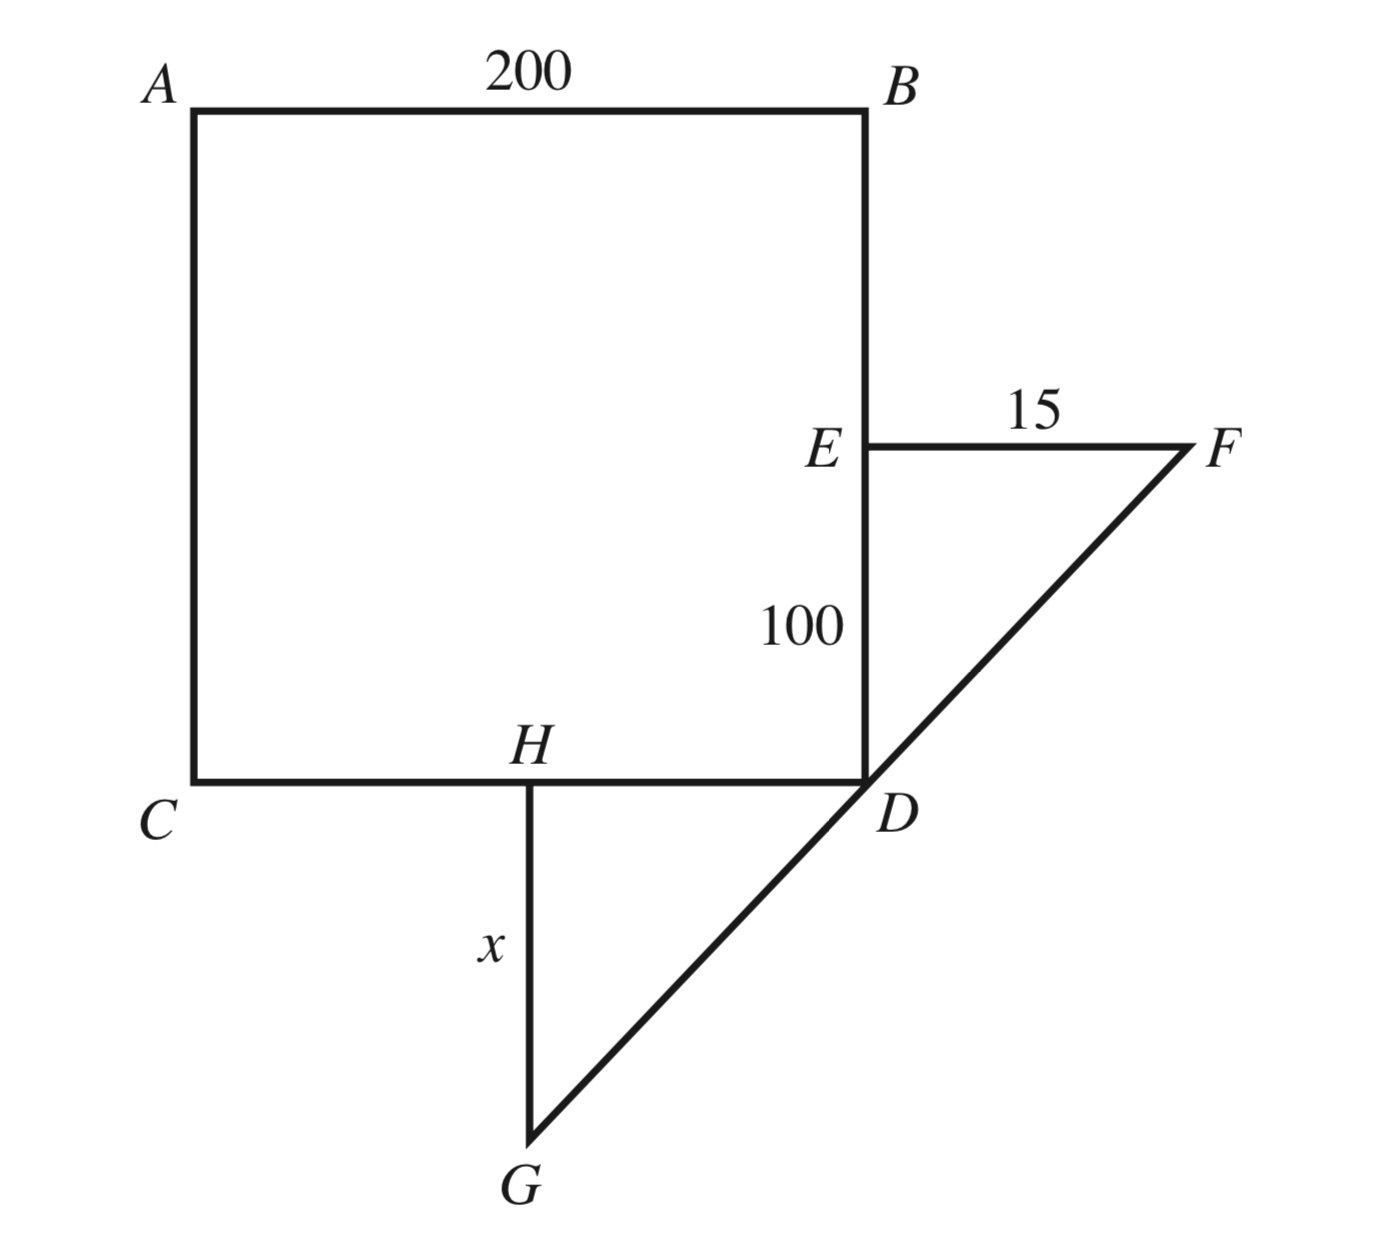
\includegraphics[ width = .55\textwidth]{squarecity.png}
    \end{center}
    \solution First consider that by construction we know that $HG || ED$, and that $\angle GHD = \angle DEF = 90$. Now 
    consider the transversal $GD$. By corresponding angles we know that, $\angle HGD = \angle EDF$. Thus by AA similarity we 
    know that $\triangle HGD \sim \triangle EDF$. Now we can solve for $x$ using the ratios from similar triangles, 
    \begin{align*}
      \frac{x}{100} &= \frac{100}{15}\\
      x &= \frac{100^2}{15}
    \end{align*}
    \vspace{.25in}

    \item A square walled city of unknown dimensions, had four gates, one at the center of each side. 
    A tree stands 20 paces form the north gate. A man walks 14 paces southward orm the south gate, then 
    turns west and walks 1775 paces before he can see the tree. What are the dimensions of the city.\\
    \begin{center}
      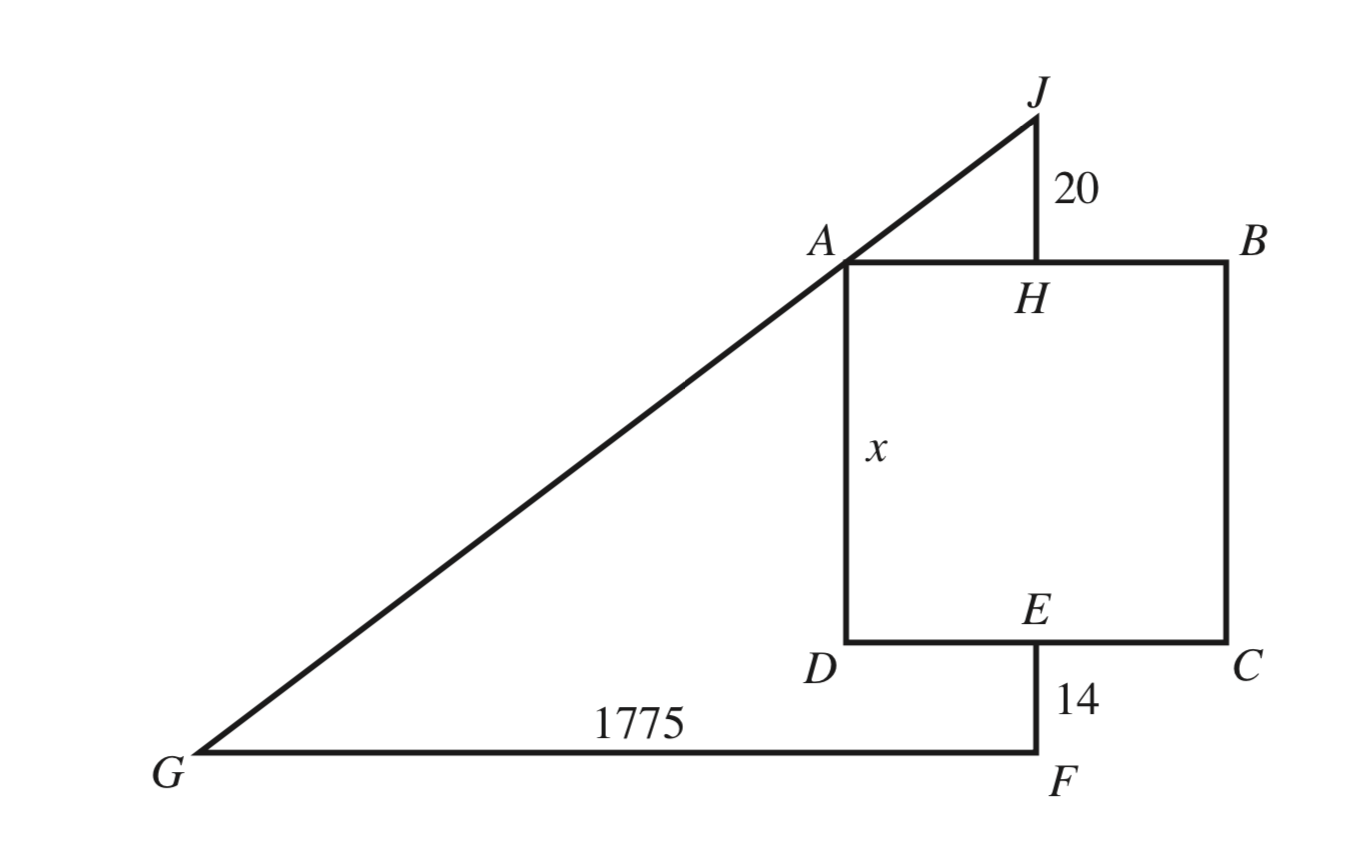
\includegraphics[ width = .55\textwidth]{squarecity2.png}
    \end{center}
    \solution Consider that by construction we know $\angle JFG = \angle JHA = 90$. Since $\triangle JHA$ and $\triangle JFG$ 
    share an angle we know that $\triangle JHA \sim \triangle JFG$ by AA similarity. Since the city is square, and the gates are at the center of each side 
    we know that $AH = \frac{x}{2}$ and $JF = 20 + x + 14$. Solving for $x$, 
    \begin{align*}
      \frac{20 + x + 14}{1775}& = \frac{(2)20}{x}\\
      x^2 + 34x &= 40(1775)\\
      x^2 + 34x - 71000&= 0\\
      (x + 284)(x - 250)&= 0
    \end{align*}
    Looking at just our positive solution we get that $x = 250$.
  \end{enumerate}
  \vspace{.5in}
\end{exercise}

  \begin{exercise}{16a} A certain number of people are purchasing chickens, jointly. If each person contributes 9 wen 
    there is a surplus of 11 wen, and if each person contributes 6 wen there is deficiency of 16 wen. Find the number of people $n$, 
    and the price of the chickens $p$.\\

    \solution Converting this problem into our notation we get the following system of equations, 
    \begin{equation*}
      9n = p + 11,
    \end{equation*}
    \begin{equation*}
      6n = p - 16.
    \end{equation*}
    Consider the same equations rewritten, 
    \begin{equation*}
      9n - p= 11,
    \end{equation*}
    \begin{equation*}
      6n - p = -16.
    \end{equation*}
    Now consider our two guesses, $n_1 = 10$ and $n_2 = 2$. Solving for $p_1$ and $p_2$ using the first equation,
    \begin{align*}
      9(10) &= p_1 + 11,\\
      p_1 &= 79.
    \end{align*} 
    \begin{align*}
      9(2) &= p_2 + 11,\\
      p_2 &= 7.
    \end{align*} 
    So our two guess pairs are $(10,79)$ and $(2,7)$. Substituting into the second equation we get, 
    \begin{equation*}
      6(10) - 79 = -19 = -16 (- 3),
    \end{equation*}
    \begin{equation*}
      6(2) - 7 = 5 = -16 (+ 21).
    \end{equation*}
    Therefore our two failures are $f_1 = -3$ and $f_2 = 21$. We know from the proof in Chapter 2 that, 
    \begin{equation*}
      n = \frac{(f_1)(n_2) - (f_2)(n_1)}{f_1 - f_2}.
    \end{equation*}
So finally we get that $n$ is, 
\begin{equation*}
  n = \frac{(-3)(2)-(21)(10)}{(-3) - 21} = 9.
\end{equation*}
Solving for $p$, 
\begin{align*}
  9(9) &= p + 11,\\
  p &= 70.
\end{align*}
\end{exercise}
\vspace{.5in}


\textbf{Additional Problems}


\begin{exercise}{1} Use the Chinese square root algorithm to find the square root of 142884.\\
  \solution Given the order of 142884 we can say that it's root can be written in the form of, 
  \begin{equation*}
    \sqrt{142884} = 100a + 10b + c. 
  \end{equation*}
  Consider $a = 3$ since $300^2 = 90000$ and $400^2 = 160000$. With $a = 3$ we calculate the remainder, 
  \begin{equation*}
    142884 - 90000 = 52884.
  \end{equation*}
  By the geometric argument in Chapter 5, $b$ must satisfy the following inequality,
  \begin{equation*}
    2(300)(10b)+(10b)^2 \le 52884.
  \end{equation*}
Finding a $b$ that satisfies $6000b \le 52884$ and then checking the inequality. Consider $b = 7$, 
\begin{equation*}
  6000(7) + (10(7))^2 = 46900 \le 52884. 
\end{equation*}
Suppose we try $8$,
\begin{equation*}
  6000(8) + (10(8))^2 = 54400 \not\le 52884. 
\end{equation*}
With $b = 7$ we calculate our remainder. 
\begin{equation*}
 52884 - 54400  = 5984
\end{equation*}
Now we need to find a $c$ that satisfies the following, 
\begin{equation*}
  2(300 + 70)c + c^2 \le 5984.
\end{equation*}
Finding a $c$ that satisfies $740c \le 5985$ and then checking the inequality. Consider $c = 8$,
\begin{equation*}
  2(300 + 70)(8) + (8)^2 = 5984 \le 5984.
\end{equation*}
Since our remainder is zero we have reached an exact answer and thus, 
\begin{equation*}
  \sqrt{142884} = 100(3) + 10(7) + 8 = 378
\end{equation*}
\end{exercise}
\vspace{.5in}

\begin{exercise}{2} Solve problem 4 from Chapter 1 of Qin Jiushao's Mathematical Treatise, which is equivalent to 
  solving this system, 
  \begin{align*}
    N &\equiv 0 \mod 11\\
    N &\equiv 0 \mod 5\\
    N &\equiv 4 \mod 9\\
    N &\equiv 6 \mod 8\\
    N &\equiv 0 \mod 7
  \end{align*}
  
  \solution To solve this problem we must first compute the product $M$, of the moduli $m_i$,
  \begin{equation*}
    M = 11*5*9*8*7 = 27720.
  \end{equation*}
  The next step involves computing all $M_i$ such that 
  \begin{equation*}
    M_i = \frac{M}{m_i}.
  \end{equation*}
  Therefore we get the following, 
\begin{align*}
  M_1 = &\frac{27720}{11} = 2520 \\
  M_2 = &\frac{27720}{5} =5544 \\
  M_3 = &\frac{27720}{9} =3080 \\
  M_4 = &\frac{27720}{8} =3465 \\
  M_5 = &\frac{27720}{7} =3960
\end{align*}

Now we reduce each $M_i$ mod $m_i$, so find a $P_i$ such that, 
\begin{equation*}
  M_i = P_i \mod m_i.
\end{equation*}
Doing that we get,
\begin{align*}
  2520 &\equiv 1 \mod 11\\
  5544 &\equiv 4 \mod 5\\
  3080 &\equiv 2 \mod 9\\
  3465 &\equiv 1 \mod 8\\
  3960 &\equiv 5 \mod 7
\end{align*}
Now we need to find one for each $P_i$ so solving for some $x_i$ that gives, 
\begin{equation*}
  P_ix_i \equiv 1 \mod m_i.
\end{equation*}
 Doing this we get, 
\begin{align*}
 (1)(1) &\equiv 1 \mod 11\\
 (4)(4) &\equiv 1 \mod 5\\
 (2)(5) &\equiv 1 \mod 9\\
 (1)(1) &\equiv 1 \mod 8\\
 (5)(3) &\equiv 1 \mod 7
\end{align*}
Finally we can compute $N$ by the following formula, 
\begin{equation*}
  N = \sum_{i}r_iM_ix_i \mod M.
\end{equation*}
We can see that for 3 of the equations $r_i = 0$ so our computation simplifies to,
\begin{equation*}
  N = 4(3080)(5) + 6(3465)(1) = 82390 = 26950 \mod 27720.
\end{equation*}
\end{exercise}
\vspace{.5in}



\begin{exercise}{3} Use the counting boards/algorithm for "finding one" to solve $88(x) \equiv 1 \mod 105$.\\
  \solution

  The counting boards/algorithm for "finding one" begins with the following, 
  \begin{equation*}
  \begin{bmatrix}
    1 && 88\\
    0 && 105
  \end{bmatrix}.
\end{equation*}
Subtracting 1 time we get,
\begin{equation*}
  \begin{bmatrix}
    1 && 88\\
    1 && 17
  \end{bmatrix}.
\end{equation*}
Subtracting 5 times we get,
\begin{equation*}
  \begin{bmatrix}
    6 && 3\\
    1 && 17
  \end{bmatrix}.
\end{equation*}
Subtracting 5 times we get,
\begin{equation*}
  \begin{bmatrix}
    6 && 3\\
    31 && 2
  \end{bmatrix}.
\end{equation*}
Subtracting 1 time we get,
\begin{equation*}
  \begin{bmatrix}
    37 && 1\\
    31 && 2
  \end{bmatrix}.
\end{equation*}
With our "one" found we get that $x = 37$, 
\begin{equation*}
  88(37) = 3256 = 105(31) + 1.
\end{equation*}
\end{exercise}
\vspace{.5in}



\textbf{Reflection}
\begin{enumerate}
  \item I definitely had to review all the algorithms that we went over last Thursday. Thankfully I was 
  able to go back and watch the class recording. 
  
  \item I though it was interesting how badly the image in the textbook portrays problem 15. $\triangle EDF$ looks 
  isosceles even though it most definitely is not.

\end{enumerate}








\end{document}